\documentclass[tikz,border=5pt]{standalone}
\usepackage[UTF8]{ctex}
\usepackage{amsmath}
\usetikzlibrary{arrows.meta,calc}
\definecolor{blue}{RGB}{45,98,142}
\definecolor{red}{RGB}{175,67,51}
\begin{document}
\begin{tikzpicture}
\draw[thick](-1.4,0)--(-1.4,-.2);
\draw[thick](-1.6,-.7)rectangle(-1.2,-.2);
\draw[thick](-1.4,-.7)--(-1.4,-1.2);
\draw[thick](-1.75,-1.2)--(-1.05,-1.2);
\draw[thick](-1.6,-1.4)--(-1.2,-1.4);
\draw[thick](-1.4,-1.4)--(-1.4,-2);
\node[left]at(-1.75,-1.3){$V_0$};\node[left]at(-1.7,-.45){$r$};
\foreach \x in{0,1.3,2.6,4.2}{\draw[thick](\x,0)--(\x,-.65);\draw[thick](\x,-1.35)--(\x,-2);}
\foreach \x in{0,1.3,4.2}{\draw[thick](\x,-1)circle(.35);\draw[thick](\x-.22,-1.22)--(\x+.22,-.78);\draw[thick](\x-.22,-.78)--(\x+.22,-1.22);\node at(\x,-2.35){$R$};}
\draw[thick](-1.4,0)--(4.2,0);\draw[thick](-1.4,-2)--(4.2,-2);
\node at(2.6,-1){$\cdots$};\node at(2.1,-2.9){共 $N$ 个相同灯泡};
\draw[blue,-{Stealth}](-.9,0)--(-.25,0)node[midway,above]{$I_N$};
\end{tikzpicture}
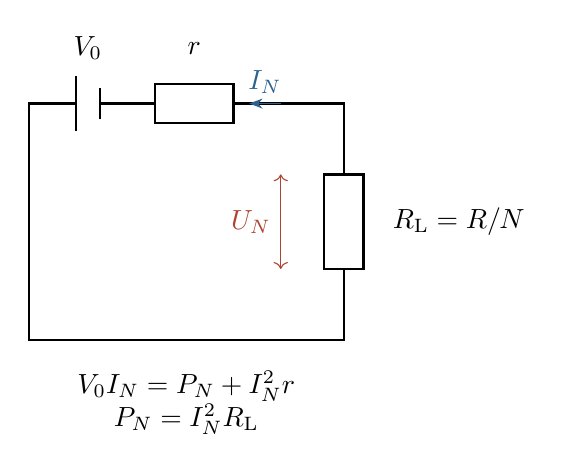
\begin{tikzpicture}
\draw[thick](0,0)--(0,1.5)--(.6,1.5);\draw[thick](.6,1.15)--(.6,1.85);\draw[thick](.9,1.3)--(.9,1.7);
\draw[thick](.9,1.5)--(1.6,1.5);\draw[thick](1.6,1.25)rectangle(2.6,1.75);\draw[thick](2.6,1.5)--(4,1.5)--(4,.6);
\draw[thick](3.75,-.6)rectangle(4.25,.6);\draw[thick](4,-.6)--(4,-1.5)--(0,-1.5)--(0,0);
\node at(.75,2.2){$V_0$};\node at(2.1,2.2){$r$};\node[right]at(4.5,0){$R_{\mathrm L}=R/N$};
\draw[blue,-{Stealth}](3.2,1.5)--(2.8,1.5)node[midway,above]{$I_N$};
\draw[red,<->](3.2,-.6)--node[left]{$U_N$}(3.2,.6);
\node[align=center]at(2,-2.3){$V_0 I_N=P_N+I_N^2r$\\$P_N=I_N^2R_{\mathrm L}$};
\end{tikzpicture}
\begin{tikzpicture}[x=.7cm,y=5cm]
\draw[-{Stealth}](0,0)--(11,0)node[right]{$N$};\draw[-{Stealth}](0,0)--(0,.31)node[above]{$P_Nr/V_0^2$};
\draw[blue,thick,domain=.01:10.5,samples=110]plot(\x,{5*\x/(5+\x)^2});
\foreach \n in{1,...,10}{\pgfmathsetmacro{\pp}{5*\n/(5+\n)^2}\fill[blue](\n,\pp)circle(1.7pt);}
\foreach \n in{4,5,6}{\draw[gray,dashed](\n,0)--(\n,{5*\n/(5+\n)^2});\node[below]at(\n,0){$\n$};}
\node[above]at(5,.25){$r=R/5$};\node[align=center]at(5.5,-.30){判据：$R^2-N(N+1)r^2$\\连续曲线仅供比较，实取正整数点};
\end{tikzpicture}
\end{document}
